\documentclass[a4,11pt,twocolumn]{article}

%%%%%% MISE EN PAGES %%%%%%
\usepackage[left=2cm, right=2cm, top=2cm]{geometry}

\setcounter{tocdepth}{3}     % Dans la table des matieres
\setcounter{secnumdepth}{3}  % Avec un numero.

%%%%%% SYMBOLES %%%%%
\usepackage{tipa}	% pour avoir l'accent concave
\usepackage{nth} 	% pour avoir first, second ... : \nth{num}

%%%%%% EQUATION %%%%%%
\usepackage{amssymb}
\usepackage{amsmath}
\usepackage{fancybox}
\usepackage{xfrac}	% fraction de type "1/4"
\usepackage{cases}	% système équation
\usepackage[overload]{empheq}
\usepackage{bm}		% pour mettre en gras .
\usepackage{units} 	% x/y barre latérale pour les fractions

%%%%%% FIGURE %%%%%%
\usepackage{graphicx}	% insérer des graphiques
\usepackage{subfigure}	% utiliser subfigure
\usepackage{float}	% utiliser H dans les figures

%%%%%% TABLEAUX %%%%%%
\usepackage{array,multirow,makecell}
\addto\captionsfrench{\def\tablename{\textsc{Tableau}}}% pour avoir TABLEAU et pas TABLE dans les légendes des tableaux
\usepackage[table,xcdraw]{xcolor} % pour avoir des lignes colorées dans les tableau
\usepackage{slashbox} % pour les \backslashbox
%\usepackage{subcaption}
\usepackage{hhline}	% pour les lignes horizontales 

\newcolumntype{L}[1]{>{\raggedright\let\newline\\\arraybackslash\hspace{0pt}}m{#1}}
\newcolumntype{C}[1]{>{\centering\let\newline\\\arraybackslash\hspace{0pt}}m{#1}}
\newcolumntype{R}[1]{>{\raggedleft\let\newline\\\arraybackslash\hspace{0pt}}m{#1}}

%%%%%%%%%%%%%%%%%%%%%
\usepackage{url}	% gérer les adresses www.
\linespread{1.2}	% interligne

\title{Creation of a corpus of realistic urban sound scenes with controlled acoustic properties}     %% \title est une macro, entre { } figure son premier argument
\author{
  GLOAGUEN, Jean-R\'emy\      \texttt{first1.last1@xxxxx.com}
  \and
  CAN, Arnaud\      \texttt{first2.last2@xxxxx.com}
  \and
  LAGRANGE, Mathieu\      \texttt{first1.last1@xxxxx.com}
  \and
  PETIOT, Jean-Fran\c cois\      \texttt{first1.last1@xxxxx.com}
}


\begin{document}

\maketitle

\section*{Abstract}
An approach is proposed to simulate a panel of urban sound mixtures from a study of recorded scenes. The aim is to succeed to compose sufficiently realistic scenes to be similar to recordings realized in cities. From a listening and recording phase, some parameters are extracted and can be used in the sound mixture simulator \textit{simScene}. The real scenes are then replicated and the realism of these are compared to the recorded scenes by a perceptive test realized on 50 people. The result prove that no particular differences can be made between the simulated and the real scenes. 

\section*{Introduction}

The urban sound environment is the subject of many researches both on perspective \cite{jin_yong_soundwalk_2013} \cite{botteldooren_understanding_2011} and on physical aspects \cite{can_describing_2015} \cite{raimbault_ambient_2003}. These studies can be based on real sound environments either by acoustic listening through a \textit{soundwalk} \cite{adams_soundwalking_2008} or with recording made in city \cite{botteldooren_temporal_2006} or in a laboratory by using sound mixtures resulting from a simulation process \cite{lafay_new_2014}. In the first case, if the urban sound environment have an undeniable ecology validity, it doesn't make it possible to have a repeatable experience nor to propose a controlled framework where the presence and the level of the different sound sources can be adjusted. Then the use of a simulation tool to create specific urban sound environments is a the only way to control the presence of each class. It allows for instance to create urban sound environments by adjusting some parameters \cite{bruce_development_2009} or to test some classification or detection tools \cite{giannoulis_detection_2013} .

The main question is then to get scenes that are realistic enough to be similar to the recordings. Various methods have been proposed. The first approach would be to simulate completely a neighborhood taking into account the architecture of the buildings, the sound dynamic of the different sources present (car, voice, bird, bell \dots) and their propagation to a receptor, as proposed by \cite{cstb_simulation_2015}. If the first renderings are interesting, this method stays complicated to implement with a final rendering that is again too artificial. 
The second approach composes sound mixtures from isolated sound associated together. The idea is to consider the urban sound environment as the sum of acoustic events, i.e events with a sufficient sound level to be discernible, superposed to a sound background, i.e a sound constant on the sound mixture whose properties vary slowly during the scene. The difficulty is to create a representative database of isolated sounds with a sufficient quality to not deteriorate the sound quality and to put the acoustic events wisely to compose correct sound environments. The method proposed in \cite{misra_musical_2007} enables to resolve the first issue by extracting the acoustical event directly in real recordings and by manipulating them to re-use them in new mixtures. If the tool has a sufficient number of parameters to control the sound event, their method is limited by the extraction phase: the overlapping between the acoustics events deteriorates the sounds and then the final rendering. In more, the manipulation (duration, frequency range) can create artifacts that can be a limitation for a realistic use. In a similar way, the tool proposed by Davis and Bruce \cite{bruce_development_2009} enables to compose sound mixtures with an isolated sound database composed of recordings made specially for their application. The creation of the urban sound mixtures is made possible with the perceptual evaluation of a panel of listeners of the different sound environments. This method enables to determine which sounds are the most representative or the most linked to an urban sound environment from a perspective point of view. 

However, as the objective is to get simulated scenes that are as realistic than recordings, this method can not be used here because if this method proposes a perspective validity it can not provide an ecological one. Thus, this study proposes to create urban sound mixtures from the listening of urban audio recordings and the estimation of some parameters extracted from them to use it in an audio simulation tool. The realism of the composed scene is then tested in a perspective test. The first part focuses on the study of a recordings made in Paris, then the second part deals with the simulation tool and the last part summarizes the result obtains in the perspective test. 


\section{Study of realistic scenes}
Real urban noise recordings are listening in details to determine the composition of typical urban sound environment in terms of sound sources, presence and level. The recordings used have been made on the \nth{13} district of Paris (France) in frame of the GRAFIC project context \cite{aumond_sound_2016} during a soundwalk which was designed to cover different types of urban sound environments. The walk was 2.1 km long, consisting of 19 stop points of 3 to 5 minutes of listening each (see figure \ref{fig:soundwalk}). It was roamed on two days (03/23/2015 and 03/30/2015) twice a day (on the morning and on the afternoon) and in one direction (from West to East, WE) and then in the other (from East to West, EW). The acquisition system used was a ASA SENS and was carry on the backpack of the operator which was walking among the participants. In the end, 74 audio in a wav format and sampled at 44,1 kHz are available and serve as a base for the study. More details can be found on  \cite{aumond_modelling_2017}. \\

\begin{figure}[H]
\centering
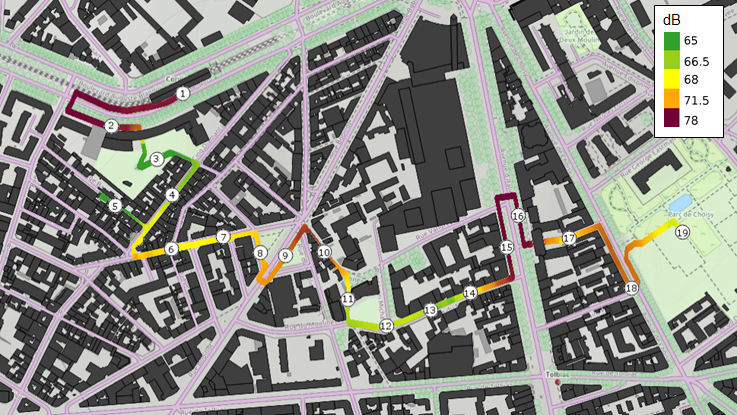
\includegraphics[width=.5\textwidth]{./pictures/trajet_19pts.png}
\caption{Map of the soundwalk with the 19 stop points}
\label{fig:soundwalk}
\end{figure}


Each audio is annotated to determine the sound classes that can be present in an urban area, their recurrence and is classified among 4 possible sound environments (\textit{park}, \textit{quiet street} , \textit{noisy street}, \textit{very noisy street}) as proposed by \cite{rychtarikova_soundscape_2013} or \cite{can_describing_2015} (table~\ref{tab:classificationScene}).

\begin{table*}[h]
\centering

\begin{tabular}{|c|c|*{19}{l|}}
\hline
\multicolumn{1}{|l|}{\textbf{day}} & \textbf{journey}   & 1                        & 2                        & 3                        & 4                        & 5                        & 6                        & 7                        & 8                        & 9                        & 10                       & 11                       & 12                       & 13                       & 14                       & 15                       & 16                       & 17                       & 18                       & 19                       \\ \hline
\multirow{2}{*}{\textbf{1}} & \textbf{EW} & \cellcolor[HTML]{F56B00} & \cellcolor[HTML]{F56B00} & \cellcolor[HTML]{5AB25A} & \cellcolor[HTML]{FFCB2F} & \cellcolor[HTML]{FFCB2F} & \cellcolor[HTML]{F56B00} & \cellcolor[HTML]{FFCB2F} & \cellcolor[HTML]{5AB25A} & \cellcolor[HTML]{F56B00} & \cellcolor[HTML]{5AB25A} & \cellcolor[HTML]{FFCB2F} & \cellcolor[HTML]{F56B00} & \cellcolor[HTML]{FFCB2F} & \cellcolor[HTML]{FFCB2F} & \cellcolor[HTML]{F56B00} & \cellcolor[HTML]{9A0000} & \cellcolor[HTML]{FFCB2F} & \cellcolor[HTML]{F56B00} & \cellcolor[HTML]{5AB25A} \\ 
\cline{2-20} 
 & \textbf{WE} & \cellcolor[HTML]{F56B00} & \cellcolor[HTML]{F56B00} &                          & \cellcolor[HTML]{FFCB2F} & \cellcolor[HTML]{FFCB2F} & \cellcolor[HTML]{FFCB2F} & \cellcolor[HTML]{FFCB2F} & \cellcolor[HTML]{FFCB2F} & \cellcolor[HTML]{F56B00} & \cellcolor[HTML]{F56B00} & \cellcolor[HTML]{FFCB2F} & \cellcolor[HTML]{F56B00} & \cellcolor[HTML]{FFCB2F} & \cellcolor[HTML]{FFCB2F} & \cellcolor[HTML]{9A0000} & \cellcolor[HTML]{9A0000} & \cellcolor[HTML]{FFCB2F} & \cellcolor[HTML]{F56B00} &  \\ 
 \hline
\multirow{2}{*}{\textbf{2}} & \textbf{EW} & \cellcolor[HTML]{F56B00} & \cellcolor[HTML]{F56B00} & \cellcolor[HTML]{5AB25A} & \cellcolor[HTML]{FFCB2F} & \cellcolor[HTML]{FFCB2F} & \cellcolor[HTML]{FFCB2F} & \cellcolor[HTML]{FFCB2F} & \cellcolor[HTML]{FFCB2F} & \cellcolor[HTML]{F56B00} & \cellcolor[HTML]{F56B00} & \cellcolor[HTML]{FFCB2F} & \cellcolor[HTML]{F56B00} & \cellcolor[HTML]{FFCB2F} & \cellcolor[HTML]{F56B00} & \cellcolor[HTML]{9A0000} & \cellcolor[HTML]{9A0000} & \cellcolor[HTML]{FFCB2F} & \cellcolor[HTML]{F56B00} & \cellcolor[HTML]{5AB25A} \\ 
\cline{2-20} 
 & \textbf{WE} & \cellcolor[HTML]{F56B00} & \cellcolor[HTML]{F56B00} & \cellcolor[HTML]{5AB25A} & \cellcolor[HTML]{FFCB2F} & \cellcolor[HTML]{FFCB2F} & \cellcolor[HTML]{FFCB2F} & \cellcolor[HTML]{FFCB2F} & \cellcolor[HTML]{FFCB2F} & \cellcolor[HTML]{F56B00} & \cellcolor[HTML]{FFCB2F} & \cellcolor[HTML]{FFCB2F} & \cellcolor[HTML]{FFCB2F} & \cellcolor[HTML]{FFCB2F} & \cellcolor[HTML]{FFCB2F} & \cellcolor[HTML]{9A0000} & \cellcolor[HTML]{9A0000} & \cellcolor[HTML]{FFCB2F} & \cellcolor[HTML]{9A0000} & \cellcolor[HTML]{5AB25A} \\ \hline
\end{tabular}

\vspace{0.5cm}


\begin{tabular}{|p{1cm}|l|p{0.001cm}|p{2cm}|l|p{0.001cm}|p{2cm}|l|p{0.001cm}|p{2.75cm}|l|p{0.001cm}|p{2cm}|l|}

\hhline{|-|-|~|-|-|~|-|-|~|-|-|~|-|-|}
park & {\cellcolor[HTML]{5AB25A}} & & quiet street & {\cellcolor[HTML]{FFCB2F}} & & noisy street & {\cellcolor[HTML]{F56B00}} & &  very noisy street & {\cellcolor[HTML]{9A0000}} & & unclassified & \\
\hhline{|-|-|~|-|-|~|-|-|~|-|-|~|-|-|}

\end{tabular}


\caption{Classification of the scenes according to the sound environment}
\label{tab:classificationScene}
\end{table*}

Most of the scene of the recordings belongs to the ambiance \textit{quiet street} and \textit{noisy street}. 2 scenes are not available : a noisy lorry sweeping the gutter is present throughout the \textit{1-WE-3} polluting the sound scene and the \textit{1-WE-19} record has been cut too quickly to be usable. From the annotation, each sound ambiance is characterized with the sound classes presents in it. The most common sound classes are resumed in the table \ref{tab:obsScene}.\\


\begin{table*}[!h]
\centering
\begin{tabular}{L{2.5cm} | C{2.5cm} | c | C{3cm} | C{2.5cm}}
\centering \textbf{Sound environment} & \textbf{Sound level (dB)} & \textbf{Background                                                       } &\textbf{Event} & \textbf{number events/min} \\ \hline
Park              & 69.0        & 
\begin{tabular}[c]{@{}l@{}}voice, \\ bird's whistles\end{tabular} & 
\begin{tabular}[c]{@{}l@{}}road traffic \\ voices\\ bird's whistle\\ street noise\\ foot step\end{tabular}                                         & 
\begin{tabular}[c]{@{}l@{}}0.5\\ 0.5\\ 0.5\\ 0.5\\ 0.3\end{tabular}                       \\\hline
Quiet street      & 70.2        & 
\begin{tabular}[c]{@{}l@{}}road traffic\\ bird\end{tabular}       & 
\begin{tabular}[c]{@{}l@{}}road traffic \\ voices\\ street noises\\ foot step\\ bird\\ \begin{tabular}[c]{@{}l@{}}construction \\ \hfill site noise \end{tabular}\\ door house\\ door car\end{tabular} & 
\begin{tabular}[c]{@{}l@{}}1.0\\ 0.7\\ 0.7\\ 0.5\\ 0.2\\ \begin{tabular}[c]{@{}l@{}} 0.1\\~\end{tabular}\\  0.2\\ 0.2\end{tabular}    
\\ \hline
Noisy street      & 73.5        & road traffic                                                      & \begin{tabular}[c]{@{}l@{}}traffic\\ foot step\\ voice\\ street noise\\ bell\\ bird\\ car horn\\ car's door\\ siren\end{tabular}                   & \begin{tabular}[c]{@{}l@{}}9.0 \\ 0.5\\ 0.6\\ 0.4\\ 0.1\\ 0.2\\ 0.3\\ 0.2\\ 0.1\end{tabular} \\ \hline
Very noisy street & 76.0        & road traffic                                                      & \begin{tabular}[c]{@{}l@{}}traffic\\ voice\\ siren\\ car horn\\ bird\\ foot step\\ car's door\\ street noise\end{tabular}                          & \begin{tabular}[c]{@{}l@{}}40\\ 0.3\\ 0.2\\ 0.3\\ 0.2\\ 0.3\\ 0.2\\ 0.3\end{tabular}      
\end{tabular}
\caption{Sound level and classes presents depending on the sound environment}
\label{tab:obsScene}
\end{table*}


%\begin{table*}[t]
%\centering
%
%\begin{tabular}{p{3cm}p{2cm}p{10.5cm}}
%\hline
%\multicolumn{1}{c}{\textbf{Ambience}} &\textbf{\begin{tabular}[c]{@{}c@{}}level\\ (dB SPL)\end{tabular}} & \multicolumn{1}{c}{\textbf{Description}} \\ \hline
%park & \centering 69,0 & predominance of children's and adults' voices and bird whistles as sound events and backgrounds, the road traffic is low almost non-existent ($\approx$ 1 car/min) \\ 
%\hline
%quiet street & \centering 70,2 & The background noise is caused by a low road traffic with few car passages ($\approx$ 2 car/min), the birds are present and audible, the voice is composed of children's and adult's voices. The effect of reverberation on the street, due to low background noise, is present.\\ 
%\hline
%animated street & \centering 73,5 & traffic noise  is louder and the unique background, the car passages density is higher ($\approx$ 10 car/min), the human activity is more present and diversify (voice, step, suitcase, construction site noise \dots), the birds disappear. \\ 
%\hline
%very noisy street & \centering 76,0 & the background noise very high composed of quasi-constant traffic flow ($\sup$ 40 car/min), the human activity are less presents in a favor of voice hubbub.\\  
%\hline   
%
%\end{tabular}
%\caption{Qualitative observations on the urban sound environment}
%\label{tab:obsScene}
%\end{table*}

The road traffic, the voice and the bird components are the most linked to the sound atmosphere: with exclusively road traffic, the sound environment is more noisy than in the \textit{park} and \textit{quiet street} where the voice and the bird's whistles are predominant. Furthermore, multiple sounds classes can be heard whatever the urban sound environments : dog barks, church bell ringing, car horn, sirens \dots with a density which can be very low (< 0.1/min). Finally, a lot of brief mechanics sounds with unknown origin can be listened in almost all the audio. Consequently, all theses indefinite sounds are classed in one unique class sound, \textit{street noise}. From theses information (density, level, sound classes present in each ambience), it is now possible to compose urban sound mixtures.

\section{Creation of realistic simulated urban scenes}
\subsection{Presentation of the web-simulator \textit{simScene}}
\textit{simScene} \cite{rossignol_simscene:_2015} is a web-simulator that creates sound mixtures in a wav format by superposing audio which comes from an isolated sound database composed of two categories: the brief sounds (from 1 to 20 seconds)
that can be salient are belong to the \textit{event} category and all the sound that are long and whose acoustic properties do not vary are put in the \textit{background} category. In each category, the sounds are then regrouping in some sound classes (bird, car, foot steps \dots). The software enables to control for each sound classes some parameters as the number of events of each class that appears in the mixture, the elapsed time between each sample of a same class or the existence of a fade in and a fade out \dots. Each parameters are completed with a standard deviation bringing some random behavior between the scenes. \\


\begin{figure}[h]
\centering
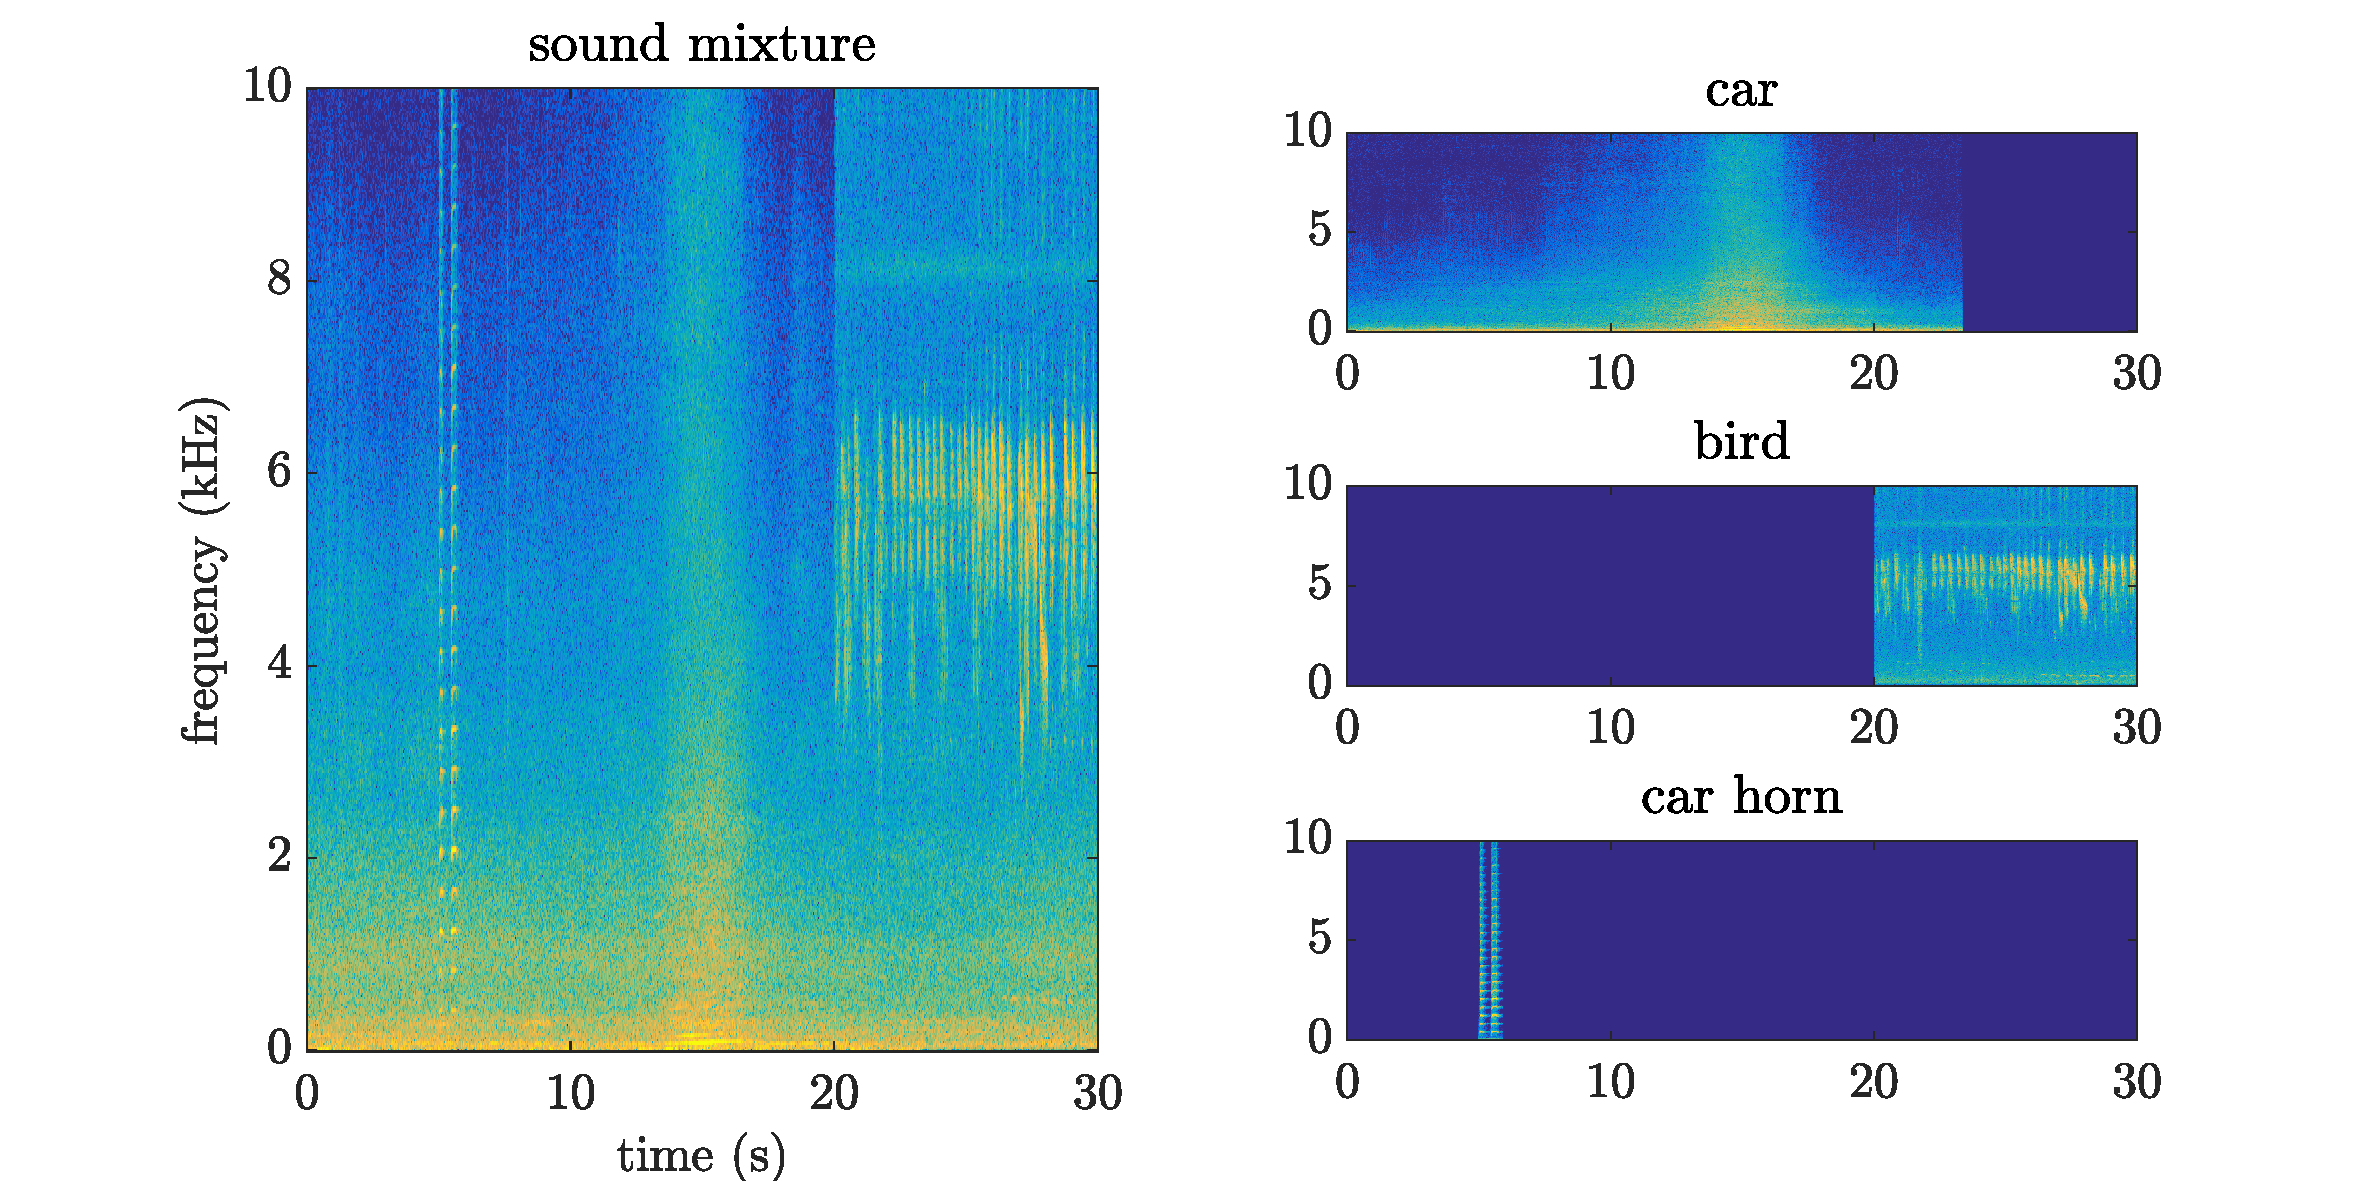
\includegraphics[width = \linewidth]{./pictures/spectrogramme_abstract_sceneSimpleKlaxonFixe_EN.pdf}
\caption{Example of a scene composed of three sound classes}
\label{fig:exampleSimScene}
\end{figure}


The sound mixtures can be create following two modes: the \textit{abstract} mode allows to create mixtures from the specified parameters while \textit{replicate} mode reproduces an existing scene from its annotation file which resumes the sound classes corresponding, their time of apparition and disappearance of every events. With the global sound mixture, an audio can also be created for each sound class present in the scene which allows to know their exact contribution in the scene. In parallel, \textit{simScene} generates 3 image files representing the temporal evolution, the spectrogram and a piano Roll representation to visualize each sound classes distribution and also two text files summarizing the temporal location of each sample and all the parameter used. \\

\subsection{Creation of the urban sound database}
Based on the annotations of the real scenes, a sound database is built with sounds found online on the \textit{freesound} project and with the urbanSound8k database\cite{salamon_dataset_nodate}. This database consists in more than 8000 files with a 4 seconds or less duration found on the web site freesound.org too, and classified in 10 sound classes : ventilation, car horn, children playing, dog barking, bell, engine idling, gunshot, jackhammer, siren and street music. All the audio have been sorted and those who presented the best signal noise ratio and are present in the sound classes identified in the real records have been selected.\\

In addition, as road traffic is a prime audio source in an urban sound environment, it seemed interesting to have, in the database, a part composed of well-recorded car audio. As a result, passages of 4 different cars (Renault Scenic, Clio, Megane and Dacia Sandero) were recorded on the Ifsttar-Nantes runway at different speeds and gear ratios for steady, acceleration and braking phases (table~\ref{tab:resum_car_audio}). In all, 103 car passages have been recorded. \\

\begin{table*}[!htb]
    \begin{minipage}{.5\linewidth}
      \centering
        \begin{tabular}{|c|c|lllll}
\cline{2-7}
\multicolumn{1}{l|}{} & \multicolumn{1}{l|}{\textbf{Trans.}} & \multicolumn{1}{l|}{\textbf{1}} & \multicolumn{1}{l|}{\textbf{2}} & \multicolumn{1}{l|}{\textbf{3}} & \multicolumn{1}{l|}{\textbf{4}} & \multicolumn{1}{l|}{\textbf{5}} \\ \hline
\multicolumn{1}{|c|}{\multirow{8}{*}{\begin{tabular}[c]{@{}c@{}}\textbf{stabilized}\\   \textbf{speed}\\   \textbf{(km/h)}\end{tabular}}} & \textbf{20} & \multicolumn{1}{l|}{$\times$} & \multicolumn{1}{l|}{} & \multicolumn{1}{l|}{} & \multicolumn{1}{l|}{} & \multicolumn{1}{l|}{} \\ \cline{2-7} 
\multicolumn{1}{|c|}{} & \textbf{30} & \multicolumn{1}{l|}{} & \multicolumn{1}{l|}{$\times$} & \multicolumn{1}{l|}{$\times$} & \multicolumn{1}{l|}{} & \multicolumn{1}{l|}{} \\ \cline{2-7} 
\multicolumn{1}{|c|}{} & \textbf{40} & \multicolumn{1}{l|}{} & \multicolumn{1}{l|}{$\times$} & \multicolumn{1}{l|}{$\times$} & \multicolumn{1}{l|}{$\times$} & \multicolumn{1}{l|}{} \\ \cline{2-7} 
\multicolumn{1}{|c|}{} & \textbf{50} & \multicolumn{1}{l|}{} & \multicolumn{1}{l|}{} & \multicolumn{1}{l|}{$\times$} & \multicolumn{1}{l|}{$\times$} & \multicolumn{1}{l|}{} \\ \cline{2-7} 
\multicolumn{1}{|c|}{} & \textbf{60} & \multicolumn{1}{l|}{} & \multicolumn{1}{l|}{} & \multicolumn{1}{l|}{} & \multicolumn{1}{l|}{$\times$} & \multicolumn{1}{l|}{$\times$} \\ \cline{2-7} 
\multicolumn{1}{|c|}{} & \textbf{70} & \multicolumn{1}{l|}{} & \multicolumn{1}{l|}{} & \multicolumn{1}{l|}{} & \multicolumn{1}{l|}{$\times$} & \multicolumn{1}{l|}{$\times$} \\ \cline{2-7} 
\multicolumn{1}{|c|}{} & \textbf{80} & \multicolumn{1}{l|}{} & \multicolumn{1}{l|}{} & \multicolumn{1}{l|}{} & \multicolumn{1}{l|}{} & \multicolumn{1}{l|}{$\times$} \\ \cline{2-7} 
\multicolumn{1}{|c|}{} & \textbf{90} & \multicolumn{1}{l|}{} & \multicolumn{1}{l|}{} & \multicolumn{1}{l|}{} & \multicolumn{1}{l|}{} & \multicolumn{1}{l|}{$\times$} \\ \hline
\end{tabular}
    \end{minipage}
    \begin{minipage}{.5\linewidth}
      \centering
\begin{tabular}{|c|c||c|c|}
\hline
\multicolumn{2}{|c||}{\textbf{braking}} & \multicolumn{2}{|c|}{\textbf{acceleration}} \\ \hline
\multicolumn{1}{|c|}{\begin{tabular}[c]{@{}c@{}}\textbf{speed}\\  \textbf{(km/h)}\end{tabular}} & \multicolumn{1}{c||}{\textbf{trans.}} & \multicolumn{1}{c|}{\begin{tabular}[c]{@{}c@{}}\textbf{speed}\\  \textbf{(km/h)}\end{tabular}} & \multicolumn{1}{c|}{\textbf{trans.}} \\ \hline
50 → 0 & 3 → 2 & 0 → 30 & 1 → 2 \\ \hline
40 → 0 & 2 → 2 & 0 → 40 & 1 → 2 \\ \hline
50 → 30 & 3 → 2 & 20 → 40 & 1 → 3 \\ \hline
60 → 40 & 4 → 3 & 30 → 50 & 2 → 3 \\ \hline
70 → 50 & 4 → 3 & 40 → 60 & 3 → 4 \\ \hline
80 → 50 & \begin{tabular}[c]{@{}l@{}}4 or 5\\ → 3\end{tabular} & 50 → 70 & \begin{tabular}[c]{@{}l@{}}3 → \\ 4 or 5\end{tabular} \\ \hline
\end{tabular}
    \end{minipage}%
    \caption{Measurement set on runway with vehicle passages with stabilized speed (left) and in acceleration and braking phase(right)} 
    \label{tab:resum_car_audio}
\end{table*}

A median filter \cite{fitzgerald_harmonic/percussive_2010} has been applied to filter out bird's whistles from the recordings in the frequency range $\left[ 2500-6500 \right]$ Hz. It   consists in taking a window around a center point and to attribute to it the median value of this window. This method allow to attenuate the brief variations both in the harmonic and the temporal plan. The size of the filter window is chosen with a 5 points width of and a 9 points height so that the effect of the filter is sufficient without deteriorating the quality of the audio (see figure \ref{fig:filtre_car}).
 
\begin{figure}[hbtp]
\centering
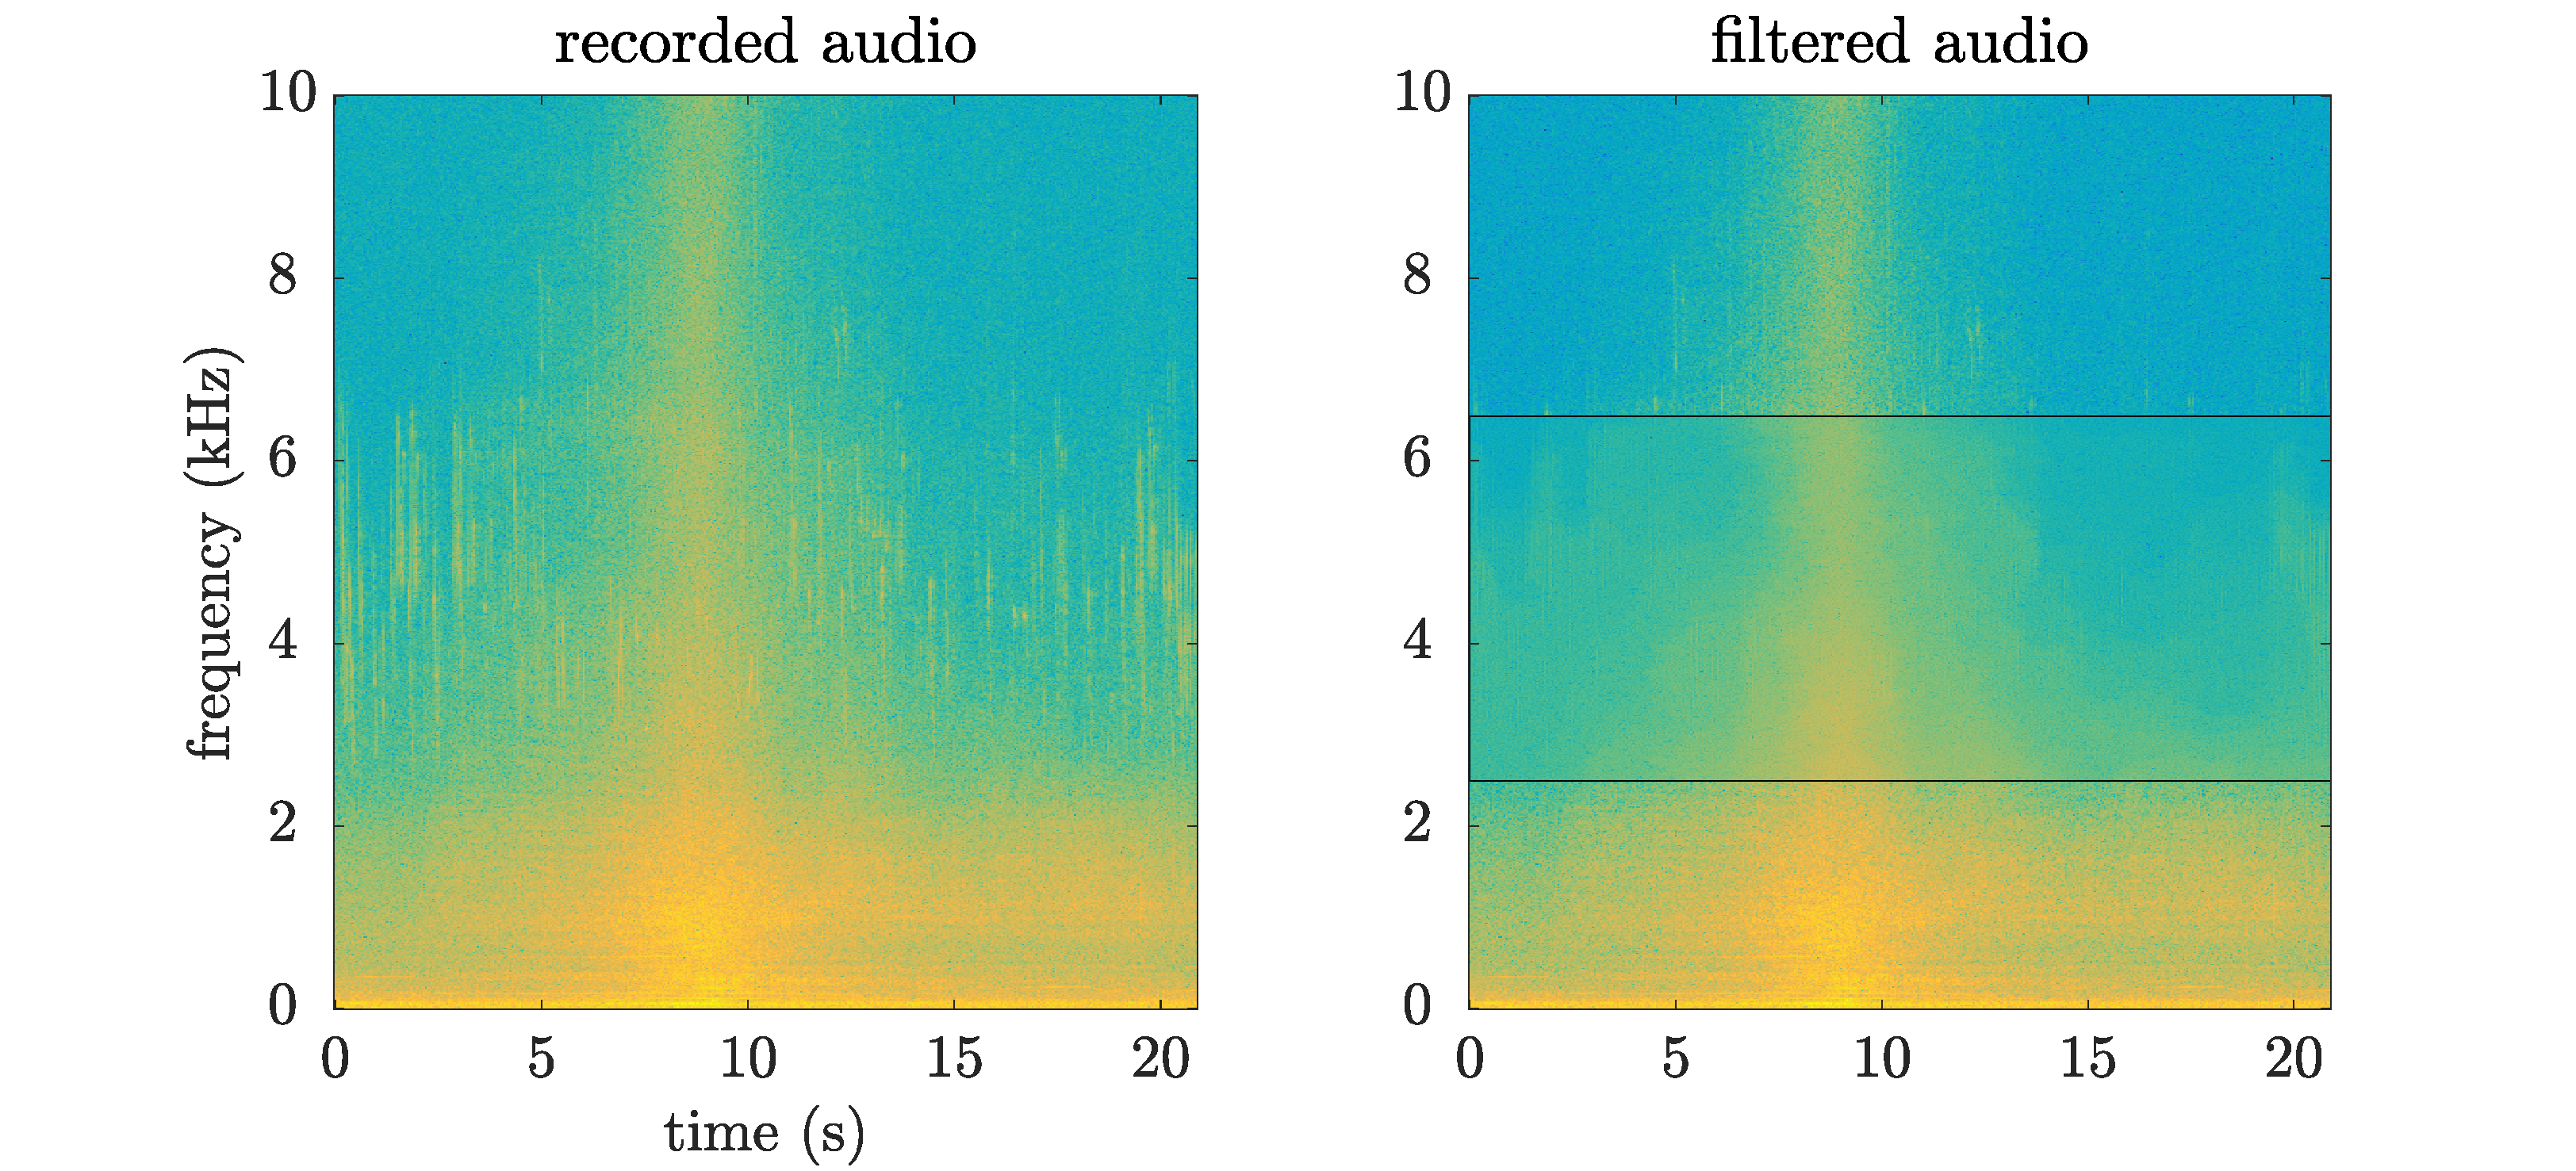
\includegraphics[width=\linewidth]{./pictures/filtrageMedian_VL1_R3_40_EN.pdf}
\caption{Spectrogram of a recorded passage of the Renault Megane car at 40 km/h with the \nth{3} gear ratio ($N_{w} = 2^{12}$ with 50 $\%$ overlapping, $N_{fft} = 2^{12}$, $sr = 44,1$ kHz). On the left, the the original recording, on the right, the filtered audio with the filtered part framed.}
\label{fig:filtre_car}
\end{figure}

Finally, the built database is composed of 245 sound events (bell, whistle bird, sweeping broom, car horn, car, hammer and drill, coughing, dog barking, car and house door slamming, plane, siren, foot step, thunder, street noise, suitcase rolling, train and tramway passing, truck and voice) and of 154 background sounds (birds, construction site, crowd, park, rain, schoolyard, traffic, ventilation, wind). With this built-up database, the 74 real sound scenes are replicated. To test whether the replicated scenes are sufficiently realistic, several of them are evaluated by a panel of listeners.

\section{Perceptual test}
\subsection{Creation of the test}
A perspective test is created where a panel of listeners evaluates the realism of a mix of real and replicated scenes on a 7-point scale (1 is \textit{not realistic at all}, 7 is \textit{very realistic}). Since it is not possible for each panelist to evaluate all the real and replicated scenes, in order to limit the duration of the test and to keep the judge's concentration constant, each listens a panel of 20 sound scenes composed of 10 real sounds scenes and 10 replicated. Furthermore, for the auditory comfort of the panelist, all the scenes are normalized to the same sound level, chosen at 65 dB.\\

First, the listening plan is elaborated following a Balanced Incomplete Block Design \cite{dagnelie_principes_2003} where $J$ participants realized $K$ evaluations from $B$ sound sources, each of them are tested $R$ times and each couple of sound sources are presented $\lambda$ times. 3 rules govern these parameters : 
\begin{subequations}\label{eq:BIE_cond}
\begin{align}
J &\geq B, \label{eq:BIE_cond1}\\
JK &= BR, \label{eq:BIE_cond2}\\
\lambda &= R\frac{K-1}{J-1}. \label{eq:BIE_cond3}
\end{align}
\end{subequations}

with $\left[J, B, K, R, \lambda\right] \in \mathbb{N}$. A reasonable number of listeners is chosen at $J = 50$ and the total numberof sound sources $B$ to be tested is set at 40. It consists of 20 30-seconds audios from the recorded scene and the same 30 seconds from the replicated scenes. Among the 20 scenes, there are 5 scenes which belong to the ambience \textit{Park}, 6 from \textit{Quiet street}, 4 from \textit{noisy street} and 5 from \textit{very noisy street} chosen randomly among the 74 scenes. As (\ref{eq:BIE_cond3}) is not satisfied, the listening plan is finally elaborated following an optimal plan \cite{pages_blocs_2007}. It consists, with the parameters $J$, $K$ and $R$ fixed, to determine the optimal plan that would be the most balanced (figure \ref{fig:repartition}).\\

\begin{figure}[ht]
\centering
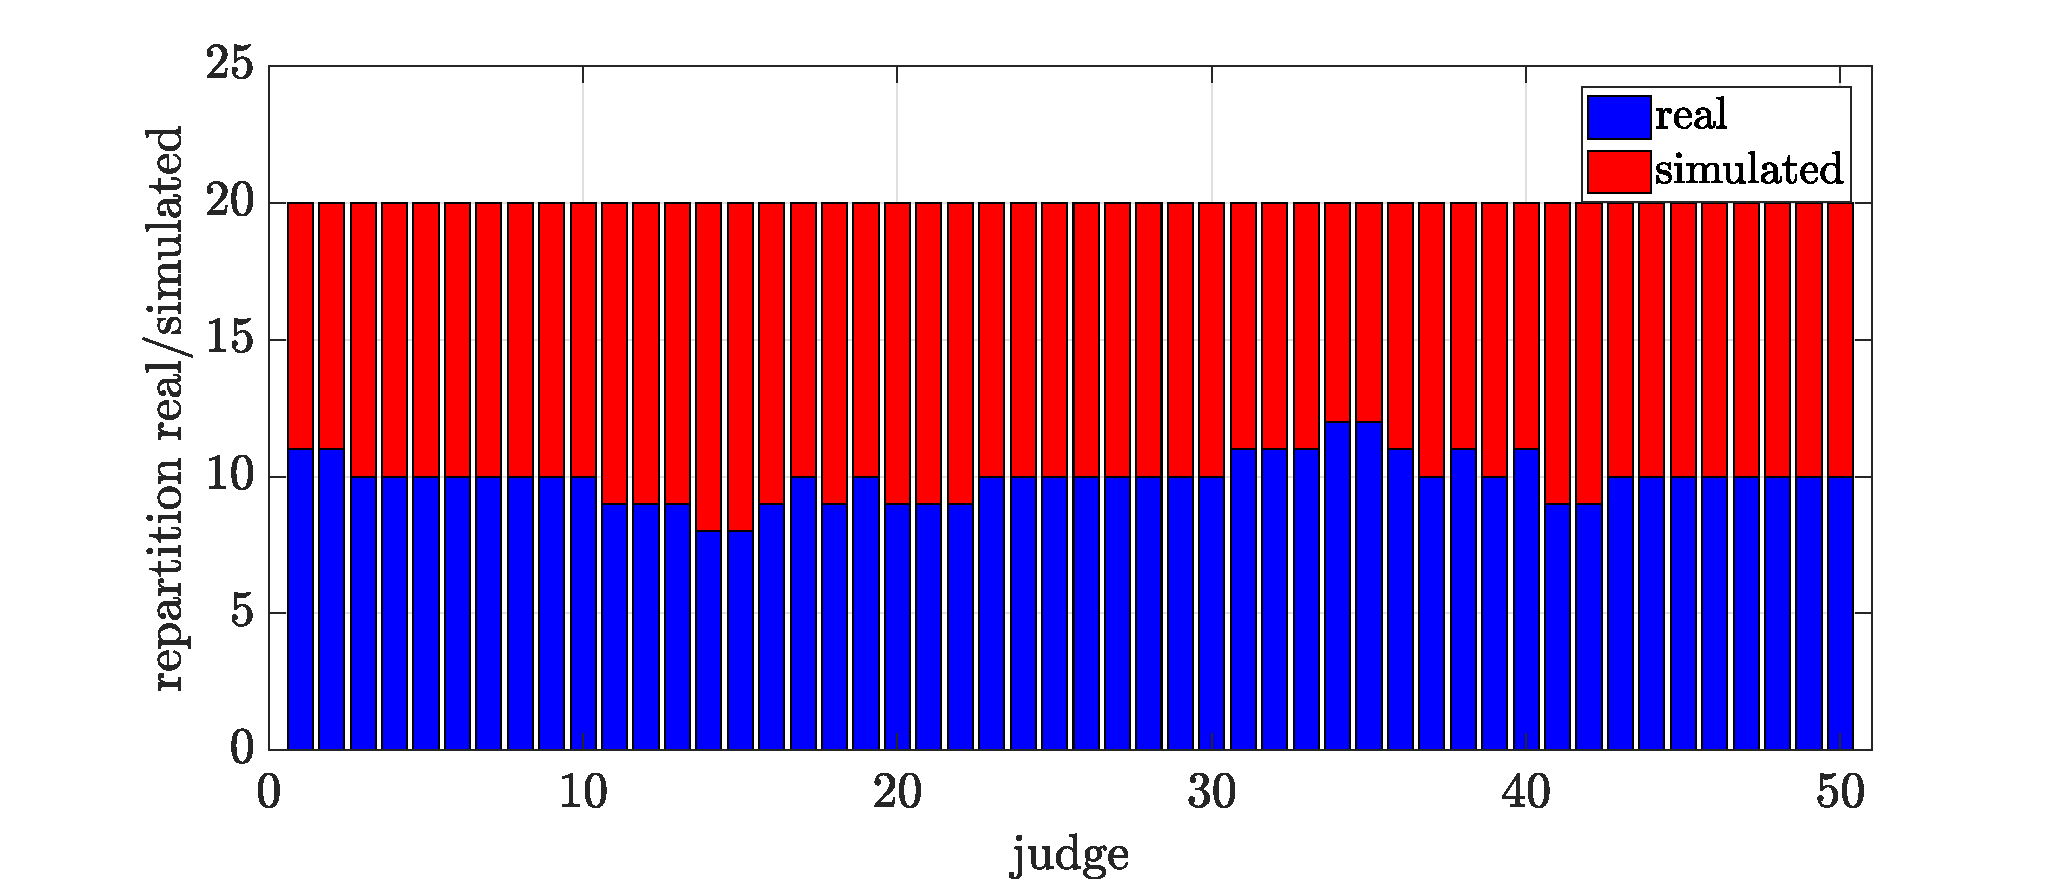
\includegraphics[width = \linewidth]{./pictures/repartition-real-simulated.pdf}
\caption{Distribution between the real and simulated scenes for each judge. The cumulative sum is equal to the number of tested elements $K$.}
\label{fig:repartition}
\end{figure}

A web-page\footnote{http://soundthings.org/research/xpRealism} was uploaded on the 8 february 2007 and the number of 50 compiled test has been reached 12 days later. During the test, the participant had the possibility to listen each scene as many time as wanted before evaluating it without being able to change his judgment afterwards. He could also leave a comment on each audio to explain his note. Finally, his age, gender and experience on listening to urban sound mixtures were asked at the end of the test. In the end, the panel of 50 listeners was made of 31 males and 18 females (one not documented) with an average age of 36 ($\pm$ 12) years old. $62\%$ of the participants declared they had no experience in the listening of urban sound mixtures.\\

%\begin{figure}[ht]
%\centering
%\includegraphics[width=\linewidth]{../../../Pictures/test_perceptif/testPerceptif_panel.pdf} 
%\caption{Description of the panel information}
%\label{fig:panel}
%\end{figure}


 
\subsection{Results}
 
An analyze of variance (ANOVA) is performed to see if both type of scenes can be discernible. 2 hypothesis are then possible : $H_0$, the real and replicates scenes can not be discernible, and $H_1$, both scenes are perceived with differences. For that, an threshold significance $\alpha=0,05$ is compared to the \textit{p-value} calculated by the ANOVA. This value represents probability to have an extreme value or more than the actual data observed considering the $H_0$ hypothesis. Two situations can happen : 
\begin{itemize}
\item $\alpha > p-value$, the $H_1$ hypothesis is validated and $H_0$ is rejected, 
\item $\alpha < p-value$, the $H_0$ is not rejected.
\end{itemize}

The data are represented by a box-and-whiskers plot according their type. 
\begin{figure}[hbtp]
\centering
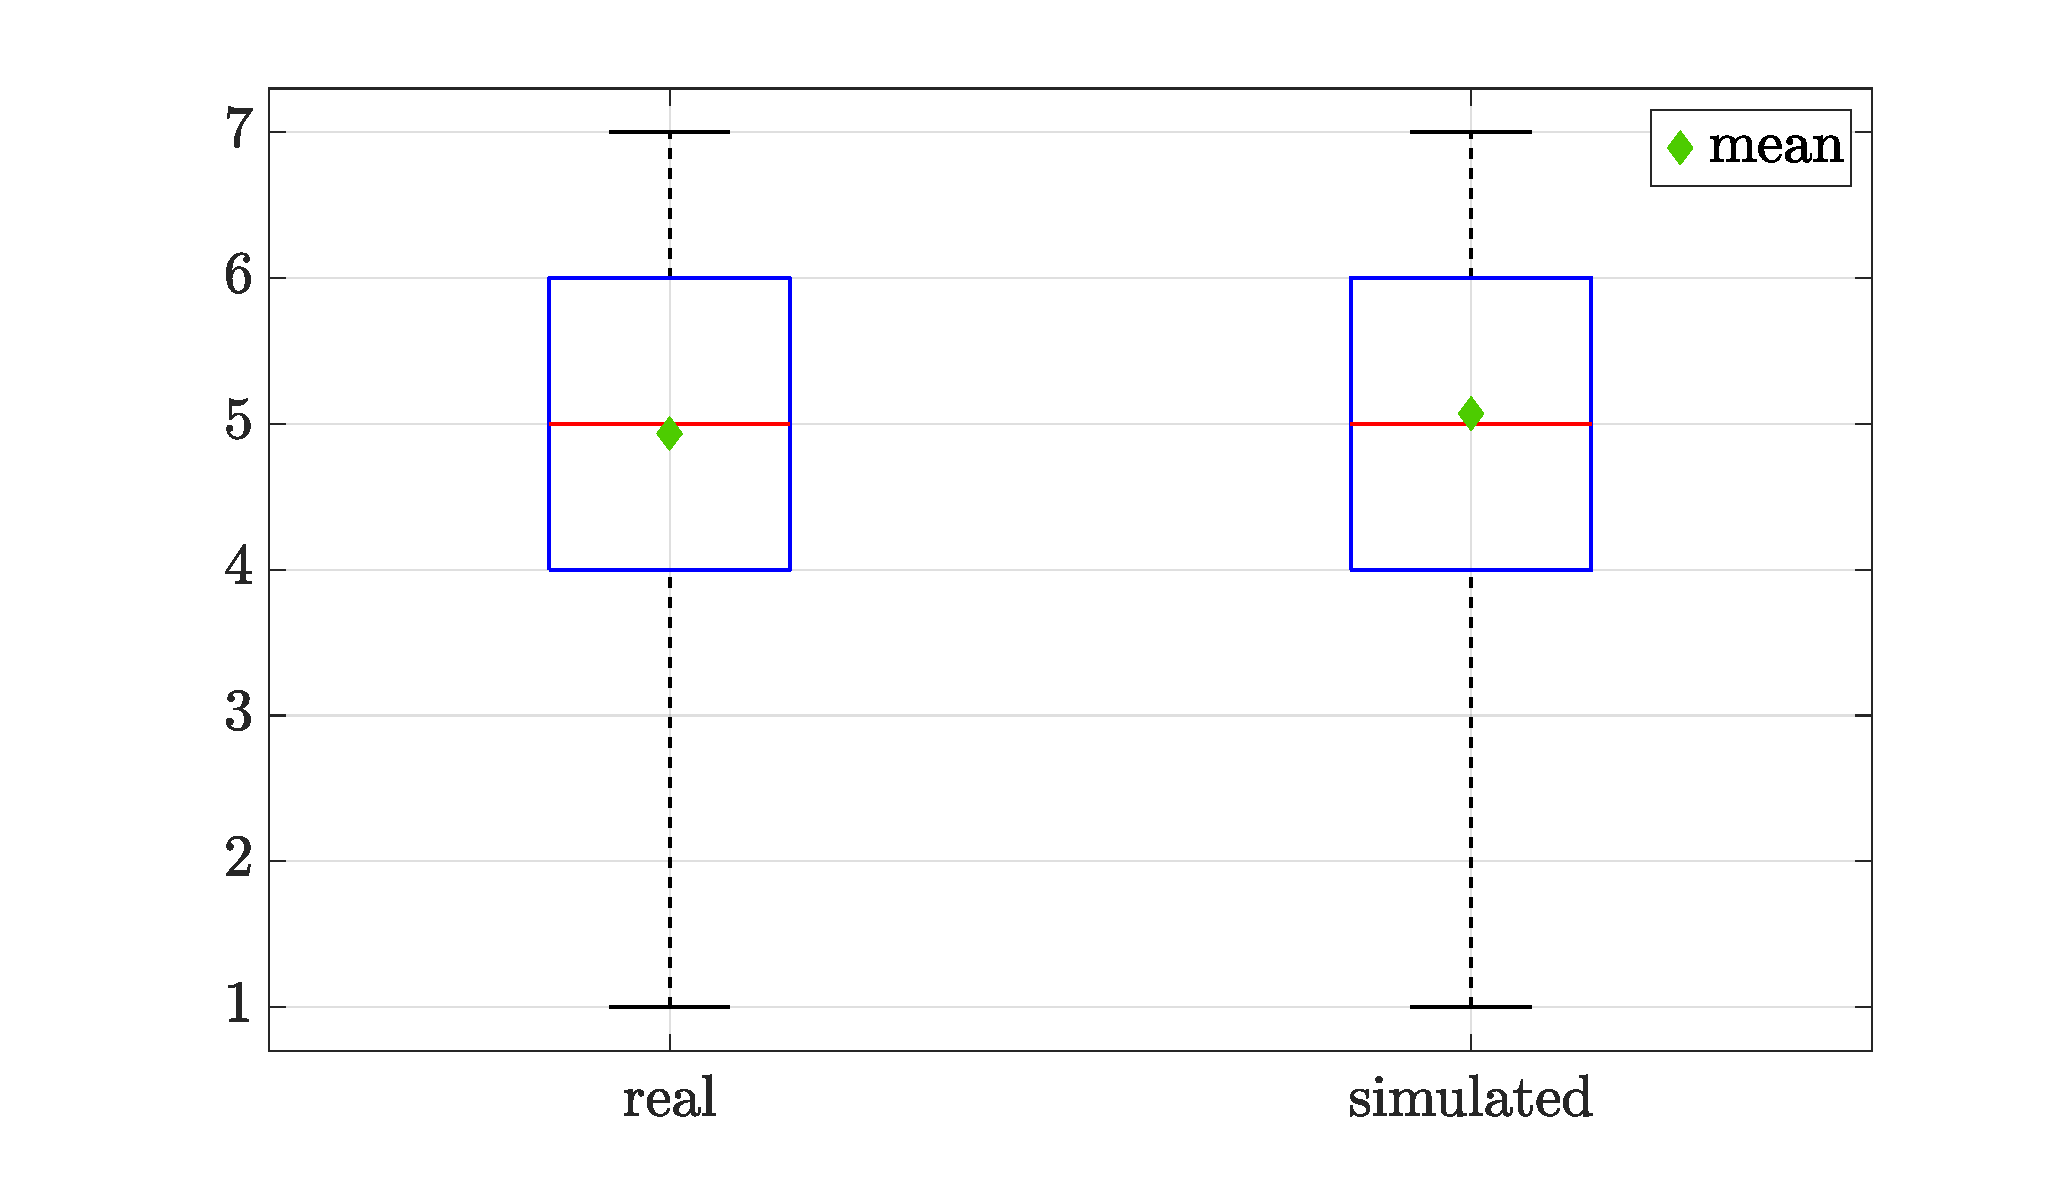
\includegraphics[width=\linewidth]{./pictures/testPerceptif_boxplotType_EN.pdf}
\caption{Box-and-whiskers plot according the type of scene}
\label{fig:boxplot_real_simul}
\end{figure}

The distribution of the note are extremely similar. The $p-value$ is calculated at $0.18 > \alpha$ which means that the two distribution cannot be distinguished. So the simulated scenes are perceived in a similar way than the recorded scenes. The mean for the simulated scene are even superior to the real ($m_{simul.} = 5.1 (\pm 1.6$), $ m_{real} = 4.9 (\pm 1.6$)). \\

Secondly, an ANOVA is performed to determine if the experience in the listening of urban sound mixtures is an influential factor to distinguish real and replicated scenes. It is then a 2 dimensions ANOVA which is used. The test allow to determine  the influence of each dimension separately and their interaction. In this case, it means that the comportment of a dimension is depending on those of the other dimension. The $p-value$ associated is submitted on the two-hypotheses test (table~\ref{tab:p_value_type_exp}).\\

\begin{table}[h]
\centering
\begin{tabular}{cccc}
\cline{2-4}
          & type & experience & interaction \\
\hline
$p-value$ & 0.50 & 0.05 & 0.17 \\
\hline    
\end{tabular}
\caption{$p-value$ for the ANOVA at two dimensions with the interaction effect}
\label{tab:p_value_type_exp}
\end{table}

The dimensions and their interaction are not significantly influential since their $ p-value $ is equal to or greater than the $ \alpha$ significance threshold. This means that even listeners trained to hear urban sound environments do not dissociate the real scenes from the simulated ones.\\

A last ANOVA is performed with 2 dimensions to see if the scenes according to the \textit{type} and their \textit{sound environment} are evaluated differently (figure~\ref{fig:boxplot_type_ambience} and table \ref{tab:p_value_type_ambience}). 

\begin{figure}[h]
\centering
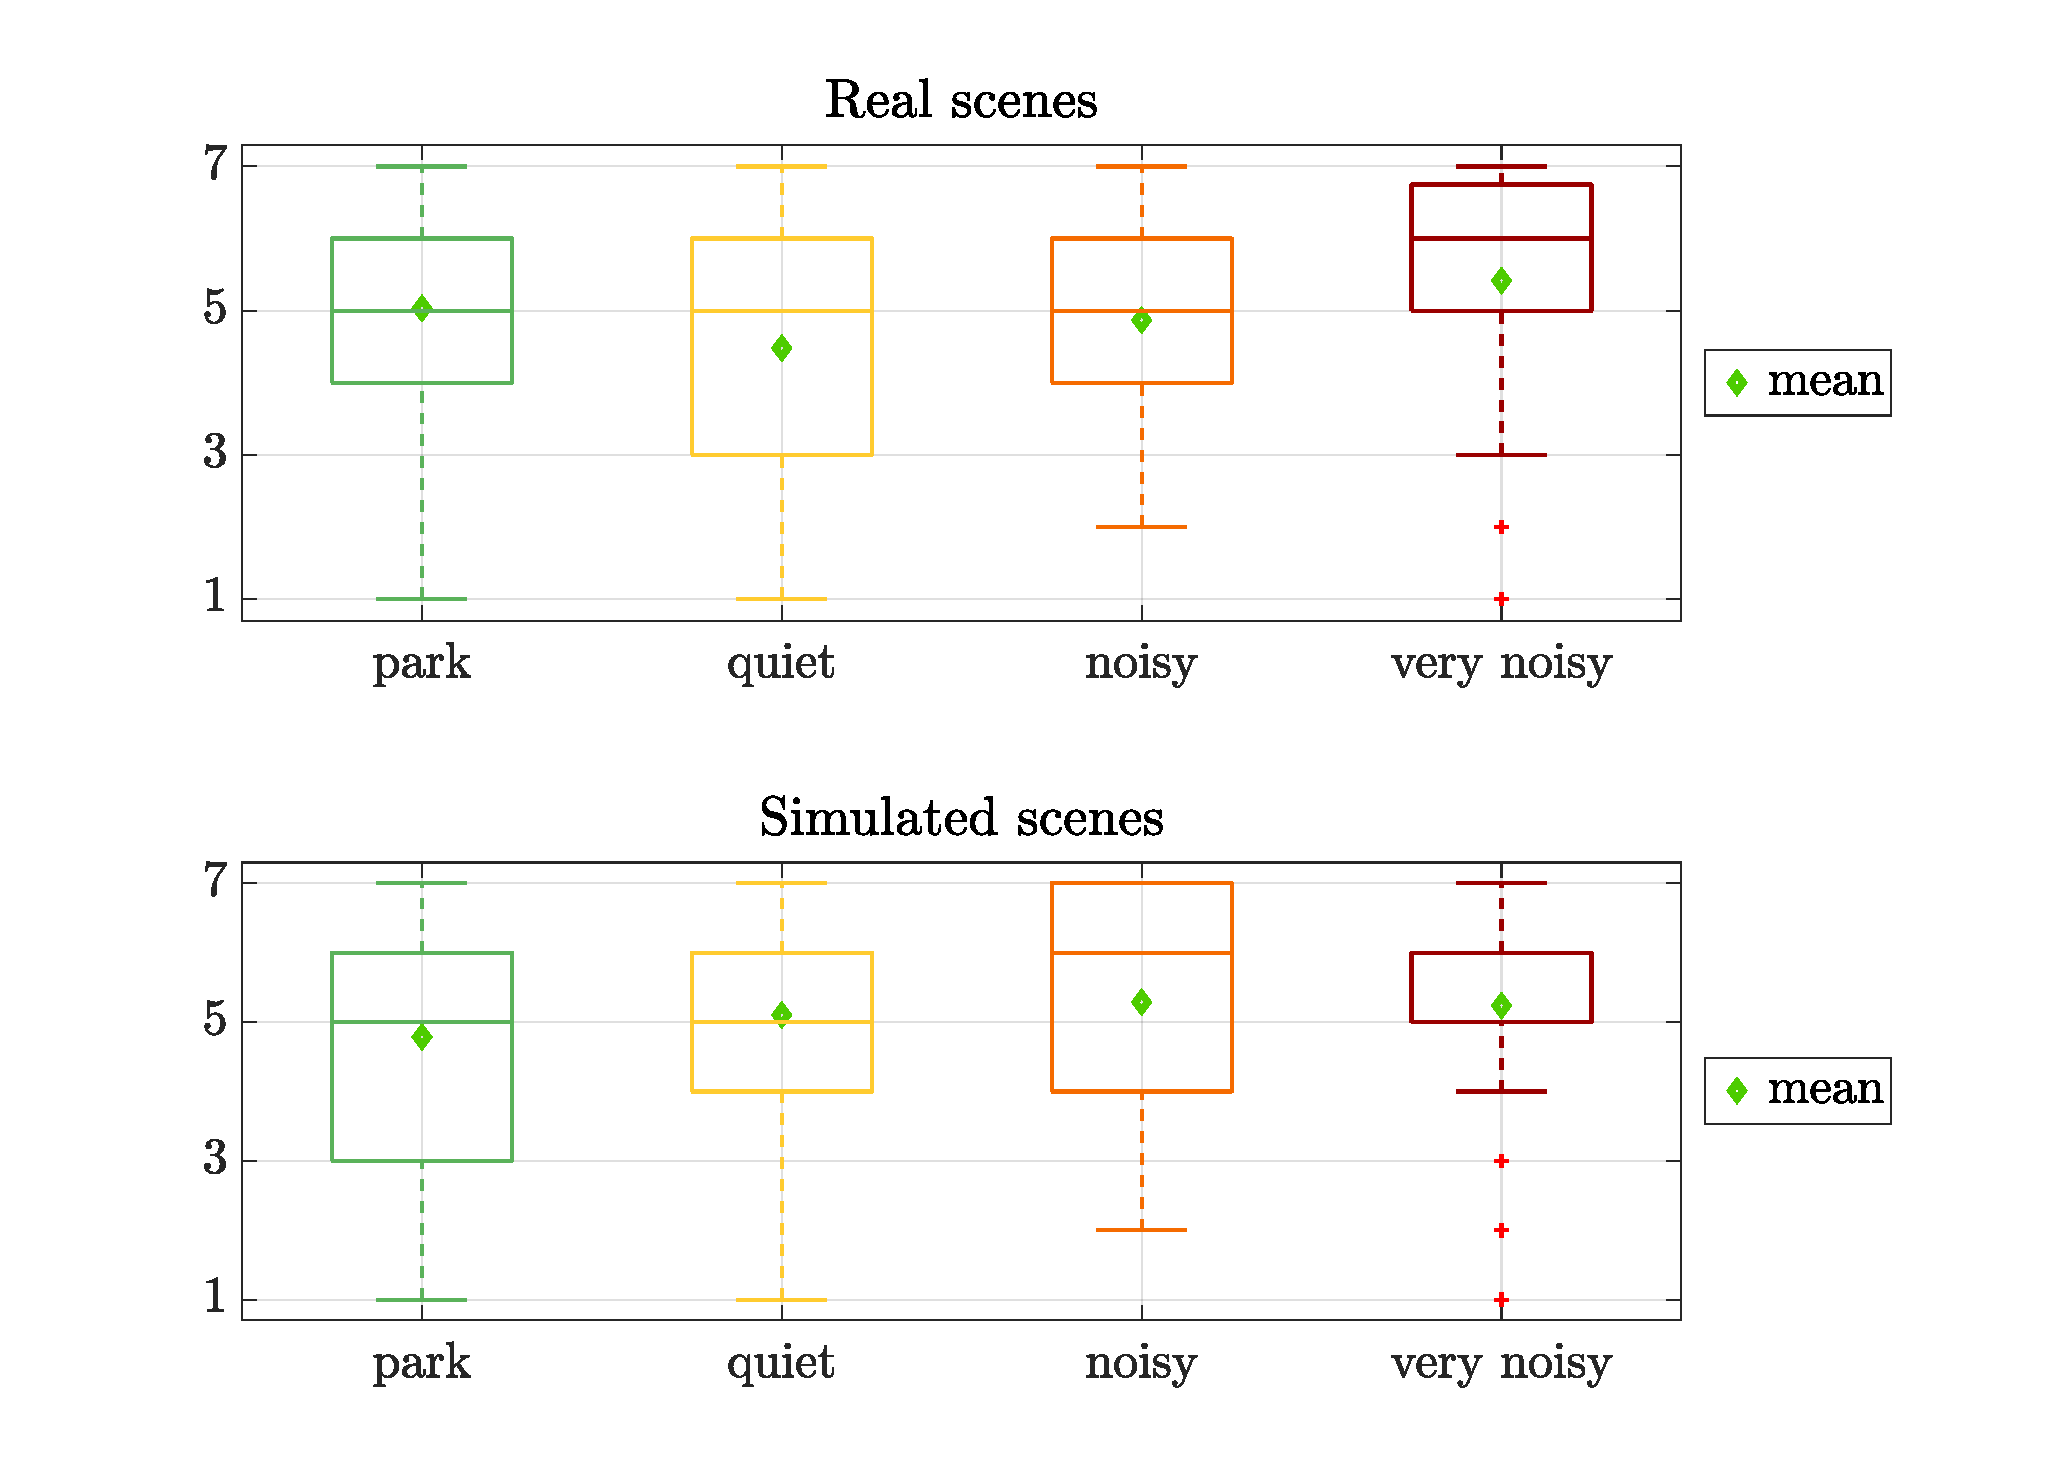
\includegraphics[width=\linewidth]{./pictures/testPerceptif_boxplotAmbianceCOLOR_EN.pdf}
\caption{Box-and-whiskers plot according the type and the sound environment}
\label{fig:boxplot_type_ambience}
\end{figure}

\begin{table}[h]
\centering
\begin{tabular}{cccc}
\cline{2-4}
          & type   & sound env. & interaction \\
\hline
$p-value$ & $0.13$ & $0.80 \times 10^{-3}$     & $2.20 \times 10^{-3}$ \\
\hline    
\end{tabular}
\caption{$p-value$ for the anova at two dimensions with the interaction effect}
\label{tab:p_value_type_ambience}
\end{table}

For the \textit{type} dimension, the effect is still not significance ($p-value > \alpha$) contrary to the \textit{sound environment} dimension. Thus, the realism of the listened scenes seems most influenced by the kind of sound environment than the type of sound scenes. As the mean of the \textit{noisy} and \textit{very noisy} atmospheres are higher, it seems that the presence of cars are a preponderant element to evaluate the realism of an audio mixture. To the opposite, for the \textit{quiet} and \textit{park} atmosphere, the evaluation is more disperse. From the comments let by the panelists, in the real scenes, the presence of too loud birds and some street noises with unknown origins have degraded the evaluation. Whereas in the simulated scenes, it is mainly the sound class \textit{foot step} and a sound background composed of birds that made the realism of the scenes decrease. \\

\section*{Conclusion}
Realistic urban sound mixtures have been composed from the study of urban recordings. A work of annotation has allowed to extract, for different acoustic atmosphere, some useful information as the sound classes presents, the traffic flow rates, the sound level. Form these observation, a urban sound database have been created including car passages recordings. A perceptual test has been set up to prove the realism of the sound mixtures. This test revealed that the replicated scenes are mistaken with the urban recordings. Furthermore, the results shows that it is more the sound environment which impact the realism than the experience of the listener. In the \textit{park} and \textit{quiet street} environment, the evaluation are more disperses and the mean note lower than the \textit{noisy} and \textit{very noisy} atmosphere. Theses differences come from mainly from the sound level of some events which are too loud to be realistic enough but that can be improved. From theses issues, it is possible to improve again the realism  of the replicated scenes by taking these comments account.

\section*{Acknowledge}
We would like to thank Pierre Aumond and Catherine Lavandier from the University of Cergy-Pontoise for transmitting us the data of the \textit{Grafic} project. 

\bibliographystyle{unsrt}
\bibliography{bibliography}

\end{document}